\section{The Intel 486}

\begin{wrapfigure}[5]{r}{0.25\textwidth}
\centering

\includegraphics[width=.25\textwidth]{drawings/intel_logo.pdf}
\end{wrapfigure}

Announced in 1989, the Intel 80486 was a performance evolution which addressed all bottlenecks of the 386. It was very expensive, at U\$900 XXX in 2018. By 1993, the chip was finally becoming affordable. It was \doom recommended CPU. Like for its predecessor (the i386 running Wolfenstein 3D), Intel offered two flavors, an SX version and a DX version (more powerful). This choice was only enabled due to manufacturing problems. The CPU integrated a Floating Point Unit but when some chips came out of the factories mostly performing but with a malfunctioning FPUs units, Intel had an idea. Instead of throwing these away, Intel sold them at a discounted price and labeled them "SX"\footnote{Later on Intel fixed there production process but they kept offering the SX since most customers prefered getting a discount instead of a FPU they had no usage of}.\\
\par
 
\drawing{486_arch}{Intel 486 architecture}

      \par

Even though the Floating Point Unit performance was drastically improved compared to the previous generation (i387), it was still a far cry of what the ALU could deliver with performances up to 20x slower. As a result, video games of the 90s did not have the luxury to use floating point arithmetics. To play \doom, a 486-SX or a 486-DX were exactly the same thing.\\
\par




If in retrospect the 486 is an unquestionable powerhouse (both in terms of performances and sales\footnote{It was still manufactured as late as 2015 for routers}), it was far from a guaranteed success when it was released. Priced at \$520\footnote{\$950 is \$1,920 in 2017, adjusted to inflation.} for the DX 
and \$258\footnote{InfoWorld Apr 29, 1991.}\footnote{\$258 in 1991 is \$469.20 in 2017, adjusted to inflation.} for the SX, the beast left a dent on a wallet. 
On top of its price, the i486 had to face internal competition from an other CPU also manufactured by Intel around the same time, the i860. Relying on an heavily pipelined superscaler architecture crushing VLIWs\footnote{Very long instruction word.}. It three units, X, Y ,and Z allowed parallel processing which rendered it incompatible with the i386 instruction set hard the potential to easily outperform a 486. Where most CPU tried to hide complexity from compiler, the i860 allowed direct access to its parallel pipeline\footnote{https://en.wikipedia.org/wiki/NEAT\_chipset}.\\
\par
\fq{Cray on a Chip\\
\par
The Intel 80860 was an impressive chip, able at top speed to perform close to 66 MFLOPS at 33 MHz in real applications, compared to a more typical 5 or 10 MFLOPS for other CPUs of the time. Much of this was marketing hype, and it never become popular, lagging behind most newer CPUs and Digital Signal Processors in performance.
The 860 has several modes, from regular scaler mode to a superscalar mode that executes two instructions per cycle and a user visible pipeline mode (instructions using the result register of a multi-cycle op would take the current value instead of stalling and waiting for the result). It can use the 8K data cache in a limited way as a small vector register (like those in supercomputers). The unusual cache uses virtual addresses, instead of physical, so the cache has to be flushed any time the page tables changes, even if the data is unchanged. Instruction and data busses are separate, with 4 G of memory, using segments. It also includes a Memory Management Unit for virtual storage.\\
\par
The 860 has thirty two 32 bit registers and thirty two 32 bit (or sixteen 64 bit) floating point registers. It was one of the first microprocessors to contains not only an FPU as well as an integer ALU, and also included a 3-D graphics unit (attached to the FPU) that supports lines drawing, Gouraud shading, Z-buffering for hidden line removal, and operations in conjunction with the FPU. It was also the first able to do an integer operation, and a (unique at the time) multiply and add floating point instruction, for the equivalent of three instructions, at the same time.\\
\par
However actually getting the chip at top speed usually requires using assembly language - using standard compilers gives it a speed closer to other processors. Because of this, it was used as a coprocessor, either for graphics, or floating point acceleration, like add in parallel units for workstations. Another problem with using the Intel 860 as a general purpose CPU is the difficulty handling interrupts. It is extensively pipelined, having as many as four pipes operating at once, and when an interrupt occurs, the pipes can spill and lose data unless complex code is used to clean up. Delays range from 62 cycles (best case) to 50 microseconds (almost 2000 cycles).}{John Bayko, University of Regina}
\par

\fq{

\begin{wrapfigure}[11]{r}{0.55\textwidth}
\centering
\scaledimage{0.55}{i860.png}
\end{wrapfigure}

...We now had two very powerful chips that we were introducing at just about the same time: the 486, largely based on CISC technology and compatible with all the pc software, and the i860, based on RISC technology, which was very fast but compatible with nothing. we didn't know what to do. so we introduced both, figuring we'd let the marketplace decide. however, things were not that simple. supporting a microprocessor architecture with all the necessary computer-related products --- software, sales, and technical support --- takes enormous resources. even a company like Intel had to strain to do an adequate job with just one architecture. and now we had two different and competing efforts, each demanding more and more internal resources. development projects have a tendency to want to grow like the proverbial mustard seed. the fight for resources and for marketing attention (for example, when meeting with the customer, which processor should we highlight) led to internal debates that were fierce enough to tear apart our microprocessor organization. meanwhile, our equivocation caused our customers to wonder what Intel really stood for, the 486 or i860?}{Andy Grove, "Only the paranoid survive".}
\bigskip
\par
In practice however the i860 never stood a chance. Impaired by its audacious yet incompatible instruction set, only its superior design could have saved sales. With compiler technology still struggling to generate fast C properly, nothing was even remotely close to generate instructions able to exploit its super scalar capability. If only Intel had been willing to build the compilers it desperately needed the i860 history could have been different.\\
\par
\trivia{Amusingly, the i860 would still play a part in Doom's development since it was used on NextDimension boards.}
\par

\par
\subsection{Performance improvements}
Charting the 486 performances against the previous 386 showed a tremendous improvement. The first obvious reasons was the raw increase of frequency. Where Intel offered up to 40 Mhz on a 386, the smaller process of the 486 allowed up to 50 Mhz, giving it an obvious advantage. But looking close at the chart, one will notice that even at equal frequency, a 486 offered more than twice the processing power of a 386.\\

\par
\begin{figure}[H]
\centering
  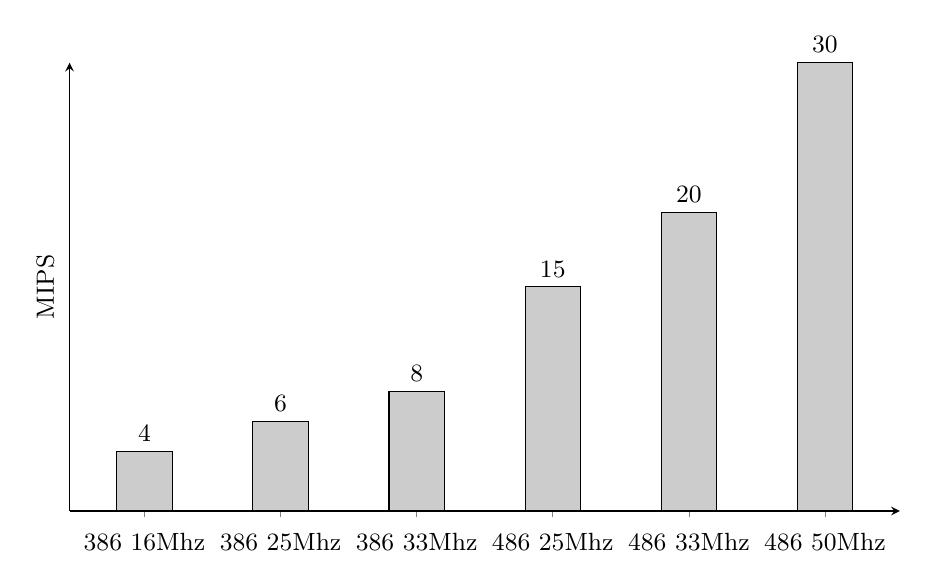
\begin{tikzpicture}[font=\small]
    \begin{axis}[
      width=1.0\textwidth,
      height=0.6\textwidth,
      ybar,
      bar width=20pt,
      ylabel={MIPS},
      ymin=0,
      ytick=\empty,
      xtick=data,
      axis x line=bottom,
      axis y line=left,
      enlarge x limits=0.11,
      symbolic x coords={386 16Mhz,386 25Mhz,386 33Mhz,486 25Mhz,486 33Mhz,486 50Mhz},
      xticklabel style={anchor=base,yshift=-\baselineskip},
      nodes near coords={\pgfmathprintnumber\pgfplotspointmeta}
    ]
      \addplot[fill=black!20,draw=black] coordinates {
        (386 16Mhz,4)
        (386 25Mhz,6)
        (386 33Mhz,8)
        (486 25Mhz,15)
        (486 33Mhz,20)
        (486 50Mhz,30)
      };
    \end{axis}
   
   \end{tikzpicture}
   \caption{Comparison\protect\footnotemark of CPUs with MIPS \protect\footnotemark.}
 \end{figure}
\footnotetext{Source: "Roy Longbottom's PC Benchmark Collection: http://www.roylongbottom.org.uk/mips.htm".}

Intel had identified all bottlenecks in the 486 and fixed them. The name of the game was to avoid ALU starvation in terms of both instructions and operands.\\
\par
\cscaledimage{0.6}{i486DX.png}{The Intel 486 packing 1.2 millions transistors.}
\par













According to Intel 80386 programmer's reference manual from 1986, their processor was a three stage pipeline which was ideally always full and busy.\\
\par
\begin{figure}[H]
\centering
\includegraphics[width=\textwidth]{drawings/386_instruction_pipeline.pdf}
\caption{386 pipeline in Intel documentation.}
\end{figure}

\par
In practice however, even if the Prefetch Unit and the Execution Unit were properly fed, the Decode unit always took a minimum of two cycles to decode an instruction\footnote{The author speculates this high decode cost was the result of Intel's choice to use CISC instead of RISC.}. Since the maximum throughput of a pipeline cannot exceed the speed of its slowest stage, the Intel 386 could process at its most one instructions every two cycles.\\
\par

\begin{figure}[H]
\centering
\includegraphics[width=\textwidth]{drawings/actual_386_instruction_pipeline.pdf}
\caption{386 pipeline: Two cycles per instruction.}
\end{figure}

\par
To solve this problem, Intel simply decided to break the three stage pipeline into four (plus an other stage explained later). With all stages performing at 1 CPI, the total throughput of the 486 was doubled.\\
\begin{figure}[H]
\centering
\includegraphics[width=\textwidth]{drawings/actual_486_instruction_pipeline.pdf}
\caption{486 pipeline: One cycle per instruction.}
\end{figure}
\par





\subsection{Caching }
Modify the pipeline and make each stage run as fast as each others was one step in the right direction. But to allow the 486 to reach and maintain maximum velocity meant to avoid the CPU stale into what Intel called Wait States.\\
\par
With the RAM located somewhere on the motherboard, the CPU must be fuelled with instructions and datas via its Bus Unit.\\
\par
\pngdrawing{cpu_chipset_bus}{}
\par
To read an address in RAM, The CPU Bus Unit asserts the 24 address lines, set the control line to "READ" and use a pin to become the bus master. This all happen in one cycle. But then the CPU has no other choice but to wait until the bus request completes. It is stuck in WAIT STATE and does nothing else. If the addressed component is fast enough, the request can complete in an second CPU cycle. Otherwise, the BUS insert more wait states \footnote{This is the same process for all I/O with the CPU. Commmunicating with the VGA or the Sound card is the same story until DMA is involved.}. From a performance perspective, WAIT STATEs are a disaster.\\
\par
\pngdrawing{cpu_wait_states}{}
From the description, even a perfect bus request with one cycle for setup and only one wait state means game over for the pipeline. To avoid using the bus as much as possible, Intel engineers added an internal cache system sitting between the pipeline and the Bus Unit.\\
\par
\pngdrawing{cpu_cache}{}




\subsection{L1 Cache}
The L1 cache was builtin the die and therefore low capacity. At only 8 KiB it may have looked tiny but its clever design and superior access time made it the real powerhouse of the 486.

\subsubsection{DRAM vs SRAM}
The first thing the cache had going on for itself is the lower latency of its RAM. If the main RAM on the SIMM slots used DRAM (Dymanic RAM) the cache was made of a different type called SRAM, able to  much faster access time. DRAM of these days typically had an access time of 150ns while SRAM was capable of 10ns, 1000\% faster.\\
\par
DRAM was "slow" grealy because it was unavailable some of the time. The design of each cells was simple, based on one transistor and one storage capacitor. Two elements allowed for tight packing and hight capacity. The problem was with the capacitor losing its charge and its bit value in the process. The only way to keep the RAM integrity was to periodically refresh it every 15$\mu s$, by sending current into the capacitor. While the refresh happened, the bit cell was unavailable.\\
\par
\spngdrawing{0.5}{DRAM}{Dynamic RAM}
The DRAM was also located somewhere on the motherboard so to access it, the CPU had to request it to its Bus Unit. Not only that was far away (in terms of physical distance), the bus had to be shared with other I/O devices.\\
\par
The SRAM in contrast was located inside the chip. There was no need for expensive bus requests. Moreover it was designed differently with no less than six transistors which did not need periodic refresh.
\par
\spngdrawing{0.5}{SRAM}{Static RAM}
\par










\subsubsection{Cachelines}
Not only the L1 cache was made of faster RAM, it was also cleverly design. Even though it had the constraints of being unified (it stores both code and data) it managed to yield an impressive 92\% hit rate\footnote{Source: "The i486 CPU: Executing Instructions in One Clock Cycle".}.\\
\par
To achieve this, Intel engineers used a four-way associative design where the $2^{32}$ address space is divided in 1,953,125 pages of 2 KiB. Within each page, 128 lines of 16 bytes (also called paragraph).\\
\par
\drawing{cacheline}{The 16 bytes in a cacheline.}
\par
The cache system is made of one directory and four banks (also called ways). Each way can store 128 cacheline and therefore has a capacity of 2 KiB. These lines of 16 bytes are the elementary unit of the cache. It only deals with what it calls cachelines.\\
\drawing{mem_to_way}{How a memory address is interpreted by the cache controller}
\par
Upong receiving a 32-bit address access request, the cache controller splits it in three fields.
\begin{enumerate}
\item Use the LINE field [0-127] to look the dictionary entry.
\item Look at the four tag in the entry, if one matches the cacheline is present in the CACHE field.
\item Check the flag F in the directory to make sure the cacheline is valid.
\item Use the OFFSET [0-15] field to access the value in the cacheline.
\item Update the flag F in the directory entry to update the LRU value.
\end{enumerate}
\par
If a value was to be written an all cacheline in the four ways are valid, the cache controller uses a LRU\footnote{Least Recently Used} to evict a cacheline.\\
\par
\drawing{cacheways}{The cache controller and its four ways (banks).}
This design allowed code and data to node evict each others in loop. The fact that four ways were rotated with LRU made this cache very efficient.\\
\par
\trivia{What about increasing to eight ways? What about sixteen? According to XXX four ways gives the best bang for the bucks. A two ways cache yields a XX\% hit rate, a four-ways XX\% hit rate but going to eight only improves the percentage to XX\% and sixteeen to XX\%. The decreasing return on investment appears vividly once one a graph.}





\subsection{Netburst}
Any cache miss within the 486 pipeline triggered the eviction of a cacheline and a full 16 bytes had to be transfered from DRAM to SRAM\footnote{The prefetcher also worked with units of 16 bytes. It retrieved and stored cacheline into a prefetch queue of 32 bytes.}. Normally this would have been a very costy operation and a huge issue for the CPU. But Intel added something called NetBurst capacity to make it all work together.\\
\par
Hit rate, ZERO WAIT STATE\\
\par
\pngdrawing{netburst}{NetBurst allows for 65\% faster cacheline filling.}







\subsection{Overdrive and Writeback}
As if the huge performance improvement of the 486 were not enough, Intel managed to top it all with the its line of 80486 OverDrive. These CPU featured a frequency multiplied which made them run two times faster than the bus\footnote{To this day, designers still try to solve the problem of having a CPU so much faster than the bus.}. The 33Mhz model CPU ran at 66Mmhz and was the golden standard until 1995. It was commonly called DX2-66 and was the absolute best to run \doom.\\
\par 
\drawing{486dx2_notm}{The best CPU to run \doom at the time.}
\par
%\trivia{Want even more performance? Not only a DX2-66 ran faster, they also came with an enhanced writeback L1 cache\footnote{The standard 486 L1 cache was writethrough with post-writes.}}

\begin{figure}[H]
\centering
  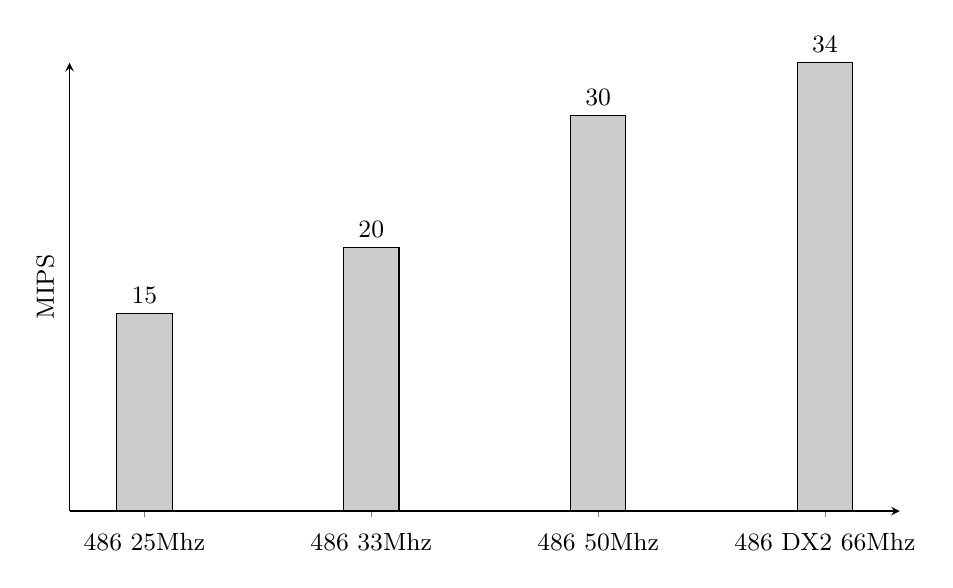
\begin{tikzpicture}[font=\small]
    \begin{axis}[
      width=1.0\textwidth,
      height=0.6\textwidth,
      ybar,
      bar width=20pt,
      ylabel={MIPS},
      ymin=0,
      ytick=\empty,
      xtick=data,
      axis x line=bottom,
      axis y line=left,
      enlarge x limits=0.11,
      symbolic x coords={486 25Mhz,486 33Mhz,486 50Mhz,486 DX2 66Mhz},
      xticklabel style={anchor=base,yshift=-\baselineskip},
      nodes near coords={\pgfmathprintnumber\pgfplotspointmeta}
    ]
      \addplot[fill=black!20,draw=black] coordinates {
        (486 25Mhz,15)
        (486 33Mhz,20)
        (486 50Mhz,30)
        (486 DX2 66Mhz,34)
      };
    \end{axis}
   
   \end{tikzpicture}
   \caption{Comparison\protect\footnotemark of CPUs with MIPS \protect\footnotemark.}
 \end{figure}
\footnotetext{Source: "Roy Longbottom's PC Benchmark Collection: http://www.roylongbottom.org.uk/mips.htm".}
\par
\trivia{Notice how a 486DX2-66Mhz is faster than a 485DX-50Mhz but not the full 20\% frequency could have made us expect. This is because the DX2 bus runs at 33Mhz while on the DX the CPU and the bus run at 50Mhz.}




\subsection{Die}
%To close this section on the 486, I cannot resist including a magnified photography of the die. 
If you are holding a physical 9.25''x7.5'' of this book, the CPU casing should be 30mm square and the die should be 15.5 x 9.9 mm at 1:1 scale.\\
\par
\bigskip

  \begin{figure}[!htb]

\begin{minipage}{0.48\textwidth}
\centering
\scaledrawimage{44.45mm}{486topdown.png}
%\caption{468 packaging.}
\end{minipage}
\hfill
\begin{minipage}{0.48\textwidth}
\centering
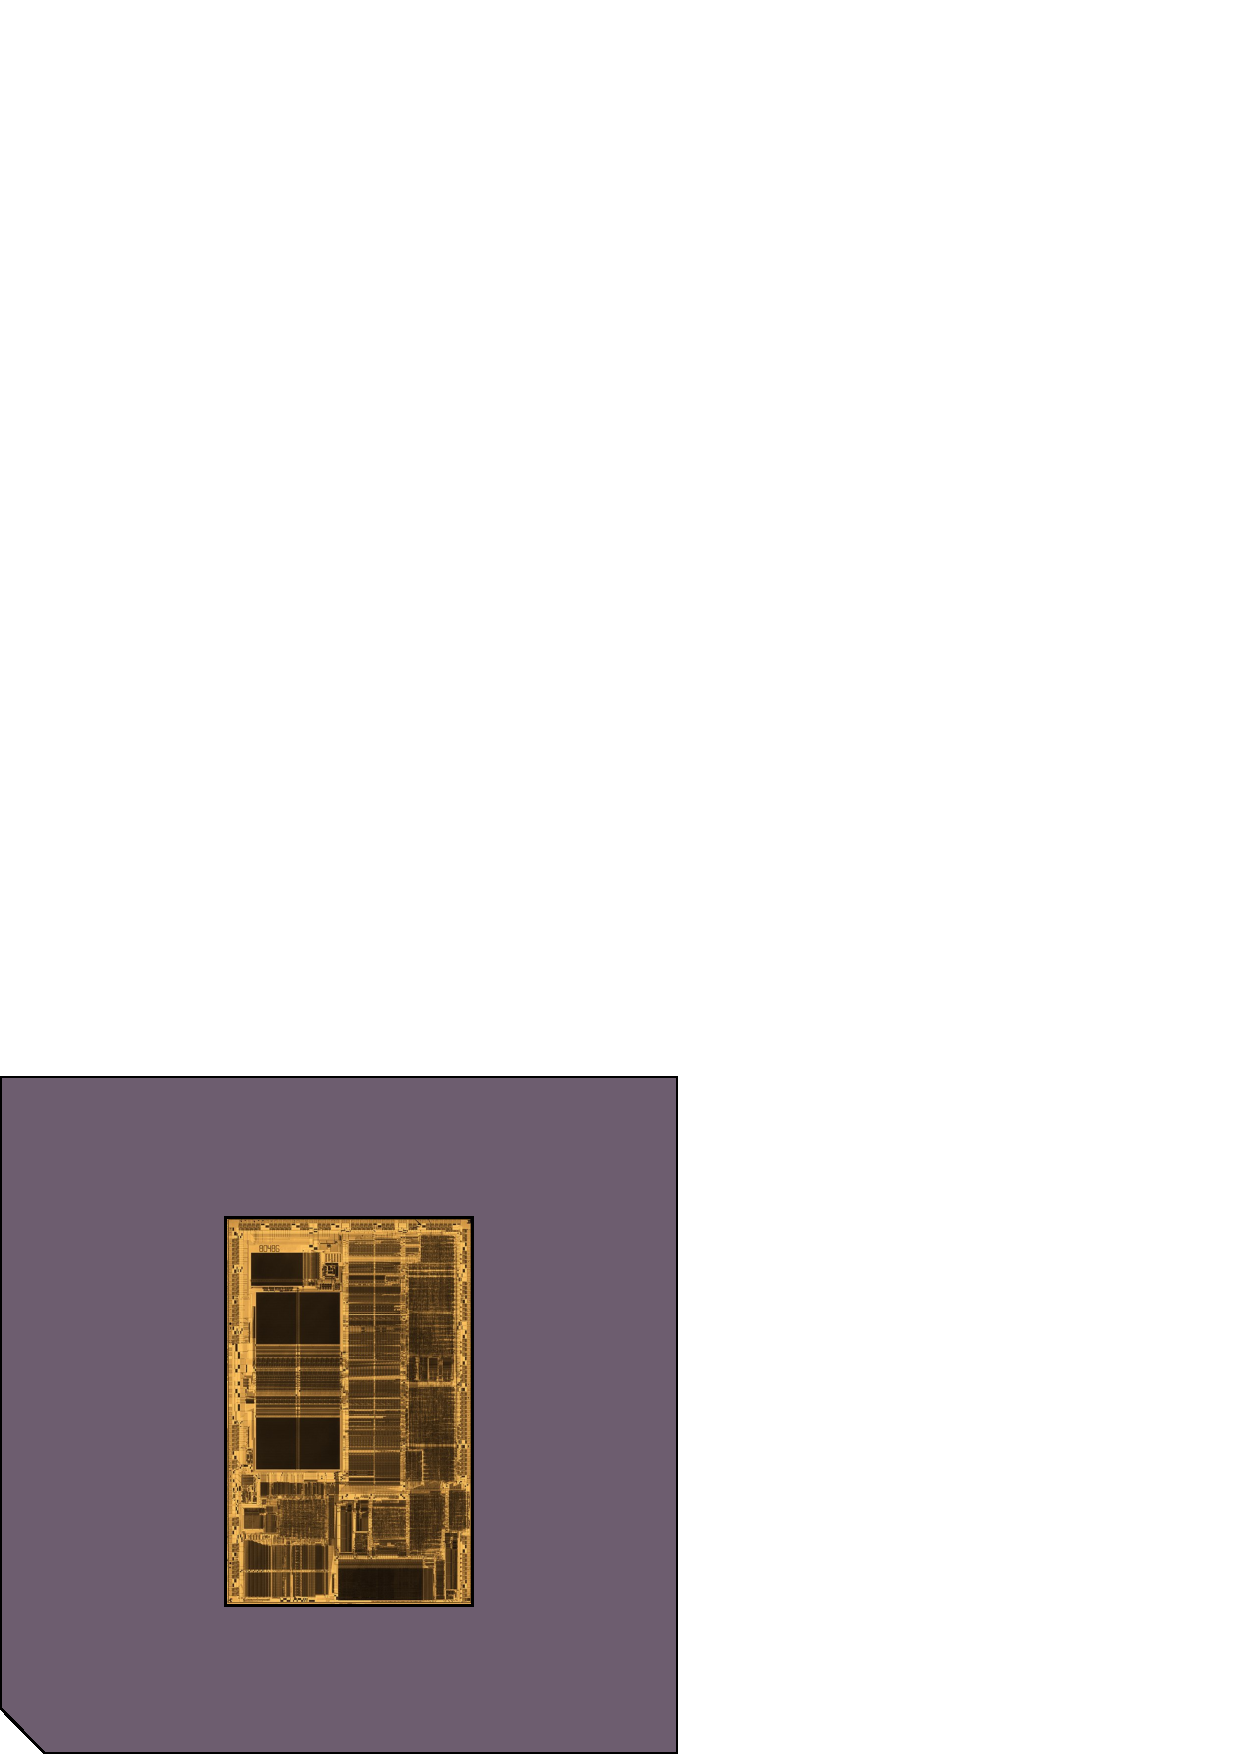
\includegraphics[width=44.45mm]{drawings/486toscale.pdf}
%\caption{The die inside the package.}
\end{minipage}
\end{figure}

\par



\begin{figure}[H]
\centering
\scaledimage{0.9}{486_blueprint.png}
\end{figure}
\par
\begin{figure}[H]
\centering
\scaledimage{0.9}{486_layout.png}
\end{figure}






\subsection{Programming the 486}
With the architecture in mind we can now understand how a programmer could take best advantage of the 486. The good news was most of the performance improvement was the characterized free-lunch of the 90s and 2000s. The exact same binary will run twice as fast on the new CPU.\\
\par
As long as the programer was mindful of the cacheline and maxmized time and space locality\footnote{And avoid branching, the 486 had no branch predictor. A \cw{jmp} instruction was a guaranteed pipeline flush}, the CPU would fly. That is for integers. Because as improved as the floating point unit was, it was still a far cry compared to the performance of the ALU and Barrel shifter.\\
\par
\begin{figure}[H]
\centering
\begin{tabularx}{\textwidth}{ X  X X  X  X}
  \toprule
  \textbf{CPU} & \textbf{FADD} & \textbf{FMUL} & \textbf{FDIV} &\textbf{FXCH} \\ \bottomrule
Intel 387 & 23-34 & 29-57   & 88-91 & 18 \\
Intel 487 & 8-20  & 16   & 73 & 4 \\ \bottomrule
\end{tabularx}
\caption{FPU performance: 387 vs 487.}

\end{figure}




\par
 \begin{figure}[H]
\centering  
\begin{tabularx}{\textwidth}{ L{0.3} L{0.3} L{0.4}}
  \toprule
  \textbf{Operation} &  \textbf{i486 (ALU)} & \textbf{i487 (FPU)} \\
  \toprule 
   
   \cw{ADD} & 1 & 8-20\\
   \cw{DIV} & 43 & 73\\
   \cw{MUL} & 12-42 & 29-52\\
   \toprule
\end{tabularx}
\caption{Comparaison ALU vs FPU operations.}
\end{figure}
\par
\trivia{There were many discussions on \cw{alt.games.doom} BBS\footnote. One endless thread in particular debated on what to get to play \doom. Should customer go for an SX, should they go for a DX which was supposed to be "faster"\footnote{\cw{alt.games.doom}: Does a 486DX run Doom faster than an SX?}. Comparing simple instruction speed for \cw{integer} and \cw{float} gives us the answer.}\\
 \par


The i386 was able to talk to an i387 located on the motherboard. Requests and responses had to transition on the bus and incurred four CPU cycles of overhead. For the i486, Intel decided to integrate the i487 FPU in the same die and improved performance by a factor 2.\\
\par
TODO: Drawing
\par

TODO: Verify with 387/487 description
TODO: How to program it? Use the cache luke and avoid branching. Re-read michael abrash guide on 486.
Full CPU Diagram.
Programming a 486